\section{Linguaggio di Interrogazione SQL}

\textbf{SQL} (Structured Query Language) è il linguaggio di riferimento per la gestione delle \textbf{basi di dati relazionali}. 
In origine l'acronimo indicava \textit{Structured Query Language}, mentre oggi viene considerato semplicemente un \textbf{nome proprio}.

SQL è un linguaggio molto completo che permette di svolgere diverse operazioni su una base di dati.


SQL consente di:

\begin{itemize}
	\item Definire la struttura di una base di dati
	\item Modificare lo schema della base di dati
	\item Inserire, modificare e cancellare i dati
	\item Eseguire interrogazioni semplici
	\item Eseguire interrogazioni complesse (interrogazioni annidate, raggruppamenti, ecc.)
\end{itemize}

Per questo motivo SQL è diviso in diversi sottolinguaggi.

\begin{itemize}
	\item \textbf{DDL (Data Definition Language)}: permette di definire la struttura della base di dati e i vincoli di integrità.
	\item \textbf{DML (Data Manipulation Language)}: permette di inserire, modificare o cancellare i dati.
	\item \textbf{DQL (Data Query Language)}: permette di interrogare la base di dati tramite query.
\end{itemize}

SQL è un \textbf{linguaggio dichiarativo}.  
Questo significa che l'utente specifica \textbf{cosa vuole ottenere}, ma non \textbf{come} il sistema deve eseguire l'operazione.

Ad esempio, quando si scrive una query SQL, si indica semplicemente il risultato desiderato.

\begin{center}
	\texttt{SELECT nome FROM Studenti WHERE voto > 25}
\end{center}

Il modo in cui la query viene eseguita è deciso automaticamente dal \textbf{DBMS}.

Una componente del DBMS chiamata \textbf{query optimizer} traduce la query SQL in operazioni interne più efficienti.  
Questo processo è nascosto all'utente e permette di esprimere interrogazioni in modo \textbf{astratto e ad alto livello}.


Nel tempo sono state definite diverse versioni dello standard SQL.

\begin{itemize}
	\item \textbf{SQL-86}: prima standardizzazione del linguaggio
	\item \textbf{SQL-89}: introduzione dell'integrità referenziale
	\item \textbf{SQL-92 (SQL-2)}: estensione significativa del linguaggio
	\item \textbf{SQL:1999 (SQL-3)}: introduzione di concetti orientati agli oggetti, trigger e funzioni
	\item Versioni successive (2003, 2006, 2008, 2011, 2016): introduzione di nuove funzionalità come supporto XML, JSON e dati temporali
\end{itemize}

Le varie versioni dello standard hanno progressivamente ampliato le capacità del linguaggio, mantenendo comunque compatibilità con le versioni precedenti.
\subsection{Clausola SELECT}
\begin{figure}[H]
	\centering
	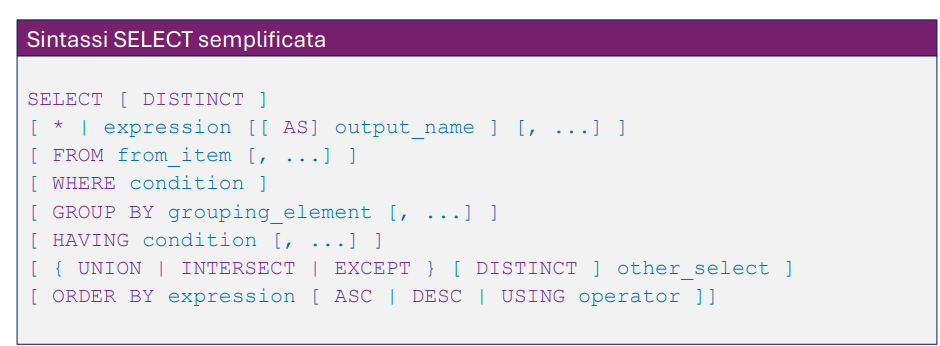
\includegraphics[width=1\linewidth]{image116}
	\caption{Sintassi SELECT}
	\label{fig:image116}
\end{figure}
\begin{itemize}
	\item \textbf{expression} è un’espressione che determina un attributo.
	\item \textbf{from\_item} è un’espressione che determina una sorgente per gli attributi.
	\item \textbf{condition} è un’espressione booleana utilizzata per selezionare i valori degli attributi.
	\item \textbf{grouping\_element} è un’espressione che permette di eseguire operazioni su più valori di un attributo e considerare il risultato complessivo.
\end{itemize}

\begin{figure}[H]
	\centering
	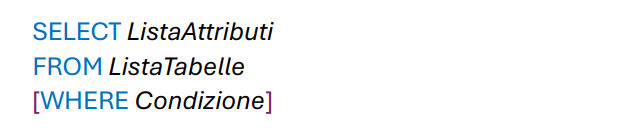
\includegraphics[width=0.7\linewidth]{image117}
	\caption{Forma semplificata SELECT}
	\label{fig:image117}
\end{figure}


\begin{itemize}
	\item \textbf{SELECT}, \textbf{FROM} e \textbf{WHERE} sono chiamate \textbf{clausole}.
	\item La query estrae dal \textbf{prodotto cartesiano} delle tabelle elencate nella clausola \textbf{FROM} le righe che soddisfano la condizione specificata nella clausola \textbf{WHERE}.
	\item Il risultato dell’interrogazione è una \textbf{tabella} con una riga per ogni riga prodotta dalla clausola \textbf{FROM} ed eventualmente filtrata dalla clausola \textbf{WHERE} (se presente).
	\item Le colonne della tabella risultante dipendono dalla lista degli attributi specificata nella clausola \textbf{SELECT}.
\end{itemize}
\begin{figure}[H]
	\centering
	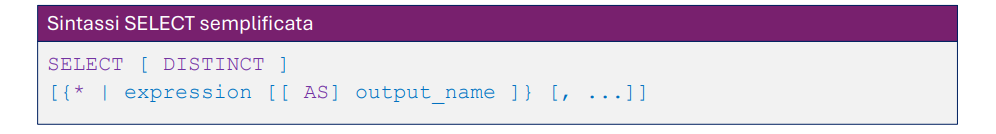
\includegraphics[width=1\linewidth]{image118}
	\caption{DISTINCT}
	\label{fig:image118}
\end{figure}
\begin{itemize}
	\item \textbf{*} è un’abbreviazione utilizzata per indicare tutti gli attributi delle tabelle.
	\item \textbf{expression} è un’espressione che coinvolge gli attributi della tabella (può anche essere semplicemente il nome di un attributo).
	\item \textbf{output\_name} è il nome assegnato all’attributo che conterrà il risultato della valutazione dell’espressione \textbf{expression} nella relazione risultato.
	\item \textbf{DISTINCT}: se presente richiede l’eliminazione delle tuple duplicate.
\end{itemize}
\begin{figure}[H]
	\centering
	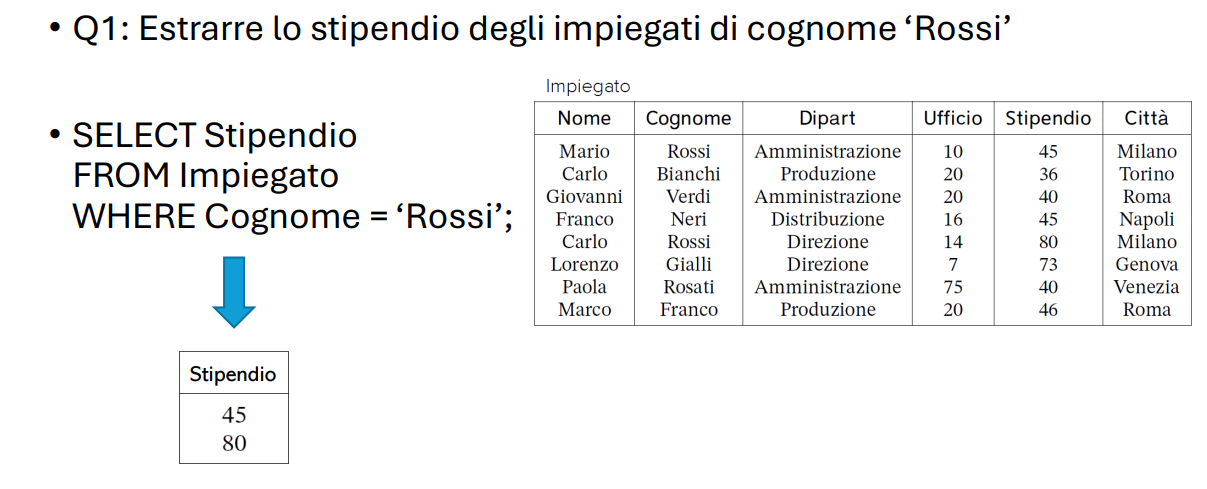
\includegraphics[width=1\linewidth]{image119}
	\caption{Esempio : Estrarre lo stipendio degli impiegati di cognome "Rossi"}
	\label{fig:image119}
\end{figure}
\begin{figure}[H]
	\centering
	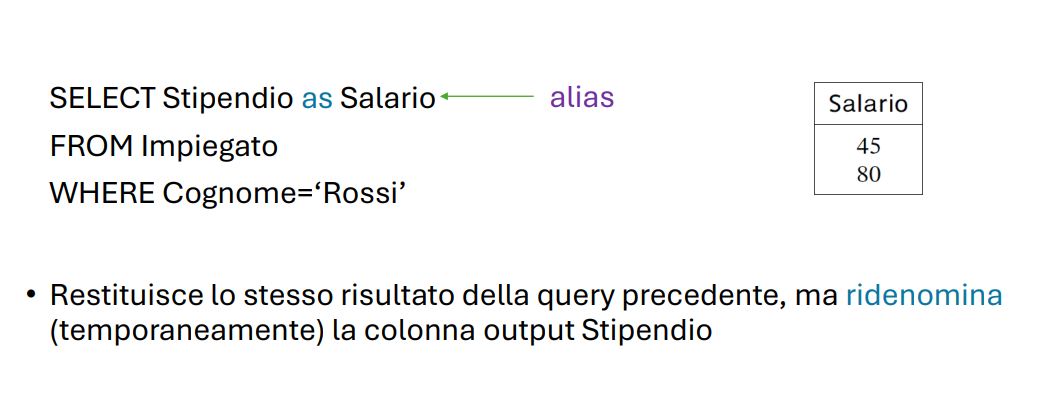
\includegraphics[width=1\linewidth]{image120}
	\caption{Uso di AS (ridenominazione)}
	\label{fig:image120}
\end{figure}
\begin{figure}[H]
	\centering
	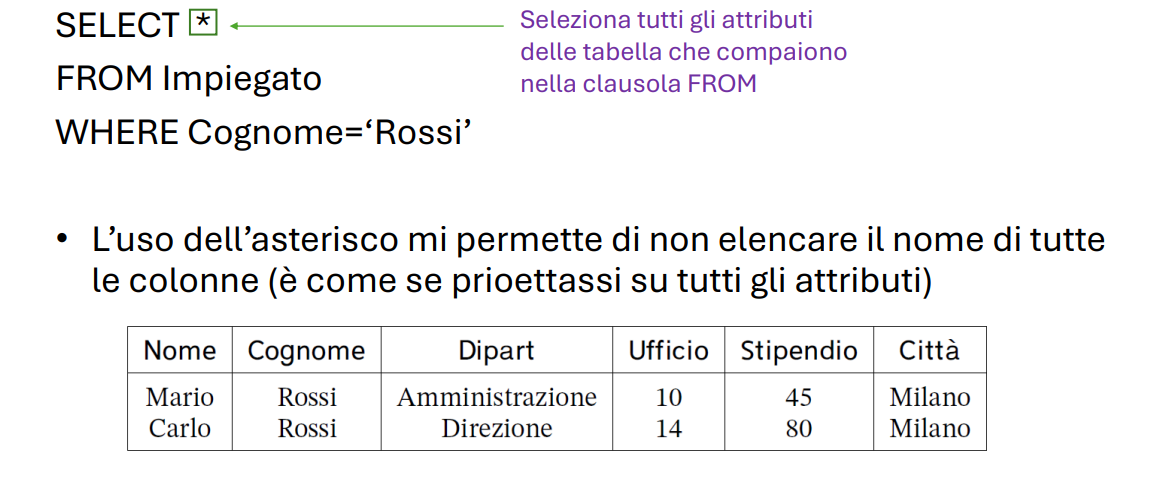
\includegraphics[width=1\linewidth]{image121}
	\caption{Uso dell'asterisco}
	\label{fig:image121}
\end{figure}
\subsection{Clausola FROM}
\begin{figure}[H]
	\centering
	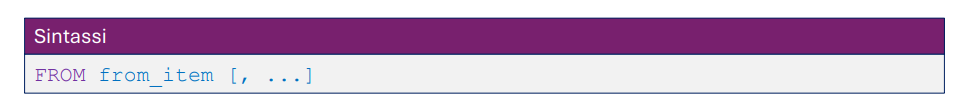
\includegraphics[width=1\linewidth]{image122}
	\caption{Sintassi FROM}
	\label{fig:image122}
\end{figure}
dove \textbf{from\_item} può essere una delle seguenti clausole (versione semplificata):

\begin{itemize}
	\item \textbf{table\_name [[AS] alias [(column\_alias [, ...])]]}
	
	Se sono presenti due o più tabelle, si esegue il \textbf{prodotto cartesiano} tra tutte le tabelle.  
	Se ci sono attributi con lo stesso nome su tabelle diverse, nella clausola \textbf{SELECT} questi attributi sono identificati anteponendo il nome della tabella e un punto:
	
	\begin{center}
		\texttt{nomeTabella.nomeAttributo}
	\end{center}
	
	\item \textbf{(other\_select) [AS] nomeRisultato [(column\_alias [, ...])]}
	
	È una \textbf{SELECT innestata}.  
	Il risultato della SELECT interna viene trattato come una tabella temporanea con nome \textbf{nomeRisultato}, sulla quale viene eseguita la SELECT esterna.
	
	\item \textbf{from\_item [NATURAL] join\_type from\_item [ON condition]}
	
	È la clausola \textbf{JOIN}.  
	
	Rappresenta un metodo più sofisticato rispetto al caso 1), che permette di selezionare un sottoinsieme del prodotto cartesiano di due o più tabelle.  
	Il parametro \textbf{join\_type} specifica il tipo di join da utilizzare. I principali tipi di join sono descritti nelle slide successive.
\end{itemize}
\begin{figure}[H]
	\centering
	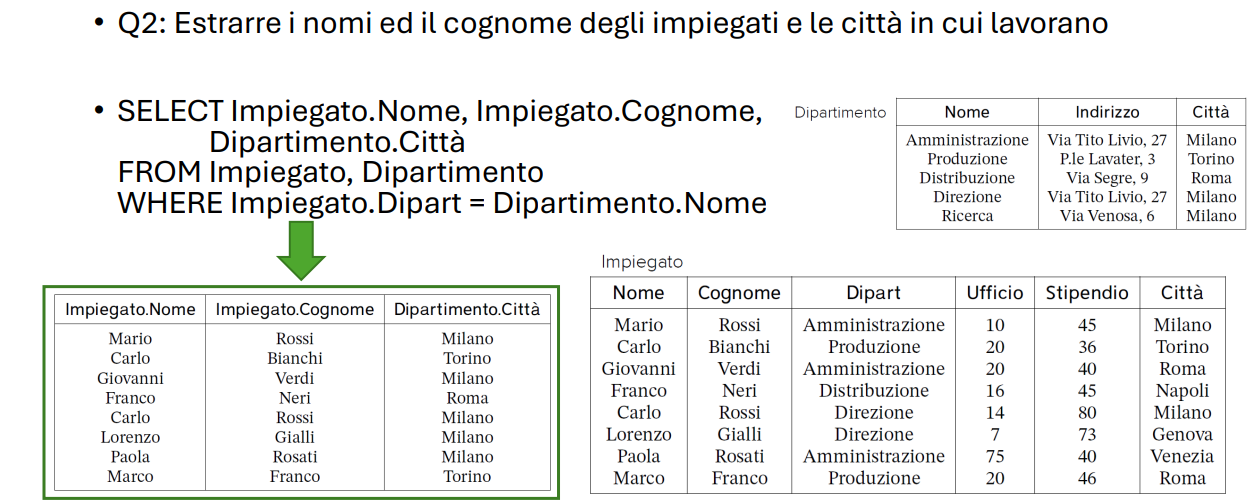
\includegraphics[width=1\linewidth]{image123}
	\caption{Estrarre i nomi ed il cognome degli impiegati e le città in cui lavorano}
	\label{fig:image123}
\end{figure}
\begin{figure}[H]
	\centering
	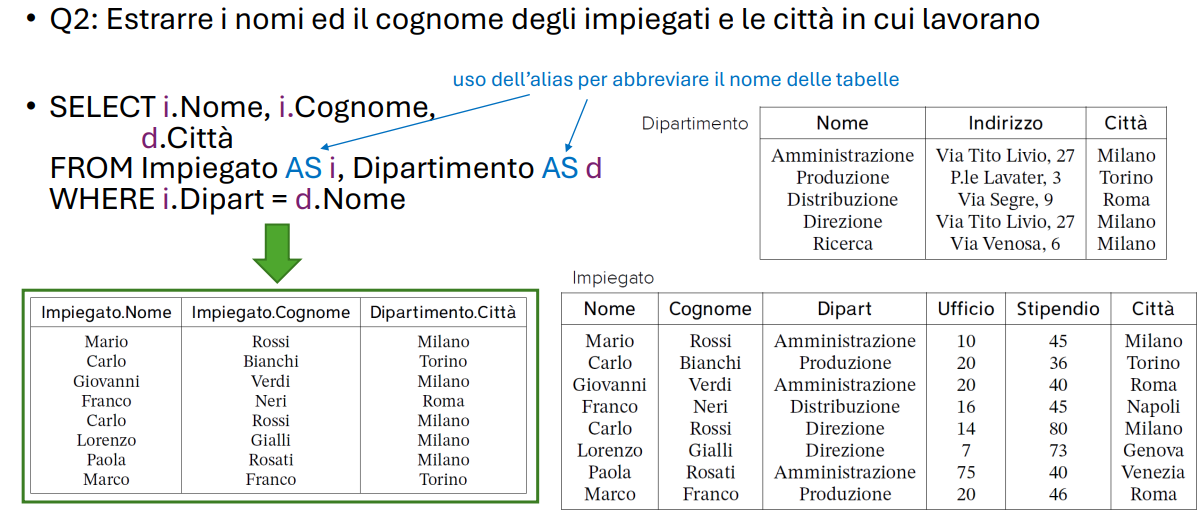
\includegraphics[width=1\linewidth]{image124}
	\caption{Stessa cosa di prima ma con AS}
	\label{fig:image124}
\end{figure}
\subsection{Clausola WHERE}
\begin{figure}[H]
	\centering
	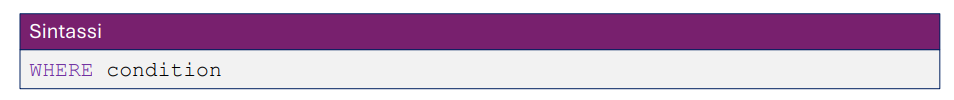
\includegraphics[width=1\linewidth]{image125}
	\caption{Sintassi WHERE}
	\label{fig:image125}
\end{figure}
\begin{itemize}
	\item La clausola \textbf{WHERE} ammette come argomento un’espressione booleana costruita combinando predicati semplici con gli operatori \textbf{AND}, \textbf{OR} e \textbf{NOT}.
	
	\item \textbf{AND}: seleziona le righe in cui tutti i predicati sono veri.
	
	\item \textbf{OR}: seleziona le righe in cui almeno un predicato è vero.
	
	\item \textbf{NOT}: seleziona le righe in cui il predicato è falso.
	
	\item Ciascun predicato semplice utilizza gli operatori \textbf{=}, \textbf{$<>$}, \textbf{$<$}, \textbf{$>$}, \textbf{$\leq$} e \textbf{$\geq$} per confrontare un’espressione costruita a partire dal valore di un attributo con un valore costante oppure con un’altra espressione.
	
	\item Per esprimere la precedenza tra gli operatori \textbf{AND} e \textbf{OR} si utilizzano le \textbf{parentesi}.
\end{itemize}
\begin{figure}[H]
	\centering
	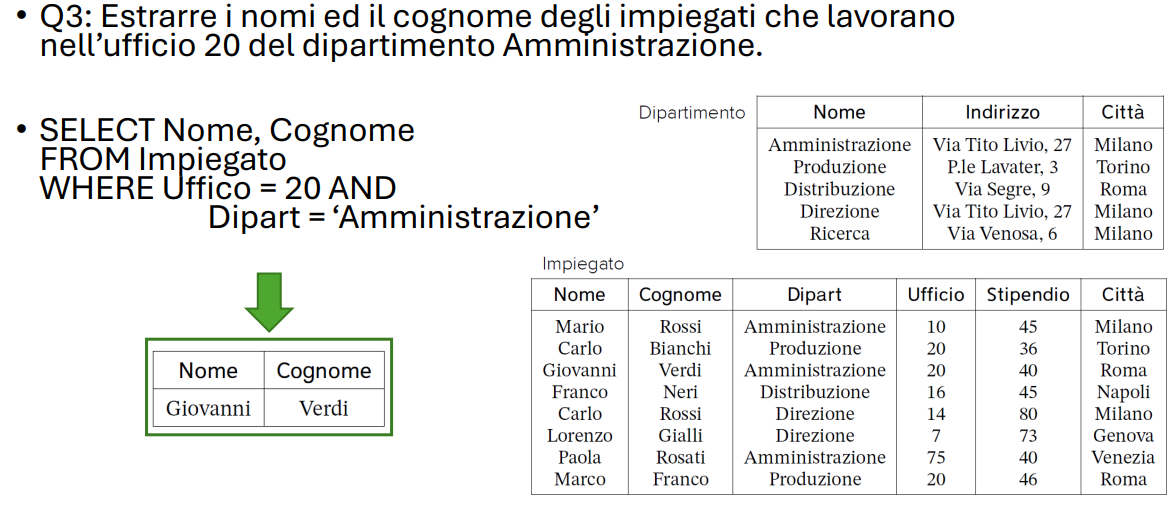
\includegraphics[width=1\linewidth]{image126}
	\caption{Estrarre i nomi ed il cognome degli impiegati che lavorano nell'ufficio 20 del dipartimento Amministrazione}
	\label{fig:image126}
\end{figure}
\begin{figure}[H]
	\centering
	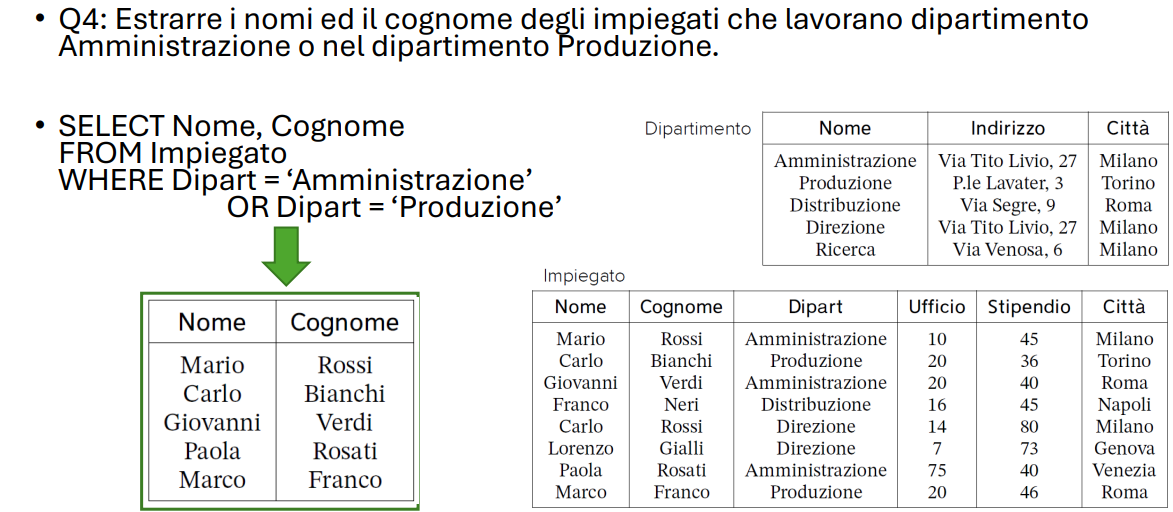
\includegraphics[width=1\linewidth]{image127}
	\caption{Estrarre i nomi ed il cognome degli impiegati che lavorano dipartimento Amministrazione o nel dipartimento Produzione.}
	\label{fig:image127}
\end{figure}
\begin{figure}[H]
	\centering
	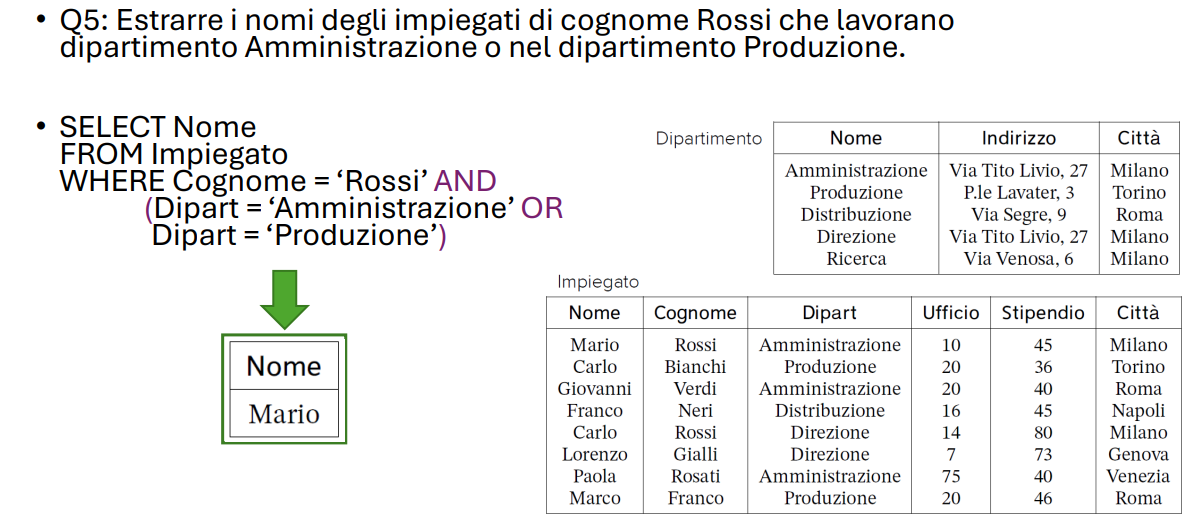
\includegraphics[width=1\linewidth]{image128}
	\caption{Estrarre i nomi degli impiegati di cognome Rossi che lavorano dipartimento Amministrazione o nel dipartimento Produzione.}
	\label{fig:image128}
\end{figure}
\subsubsection{Operatore LIKE}
\begin{itemize}
	\item Per il confronto tra stringhe, SQL mette a disposizione anche l’operatore \textbf{LIKE}, che consente di verificare se una stringa rispetta un certo \textbf{pattern} (oppure \textbf{ILIKE} per confronti \textit{case insensitive}).
	
	\item Due caratteri speciali utilizzati nei pattern sono \textbf{\_} e \textbf{\%}:
	
	\begin{itemize}
		\item \textbf{\_}: rappresenta un singolo carattere arbitrario.
		\item \textbf{\%}: rappresenta una sequenza di lunghezza arbitraria (anche nulla) di caratteri arbitrari.
	\end{itemize}
	
	\item Ad esempio:
	
	\begin{center}
		\texttt{\_o\%i}
	\end{center}
	
	rappresenta una stringa che ha una \textbf{o} in seconda posizione, seguita da una sequenza qualsiasi di caratteri (anche vuota) e che termina con una \textbf{i}.
\end{itemize}
\begin{figure}[H]
	\centering
	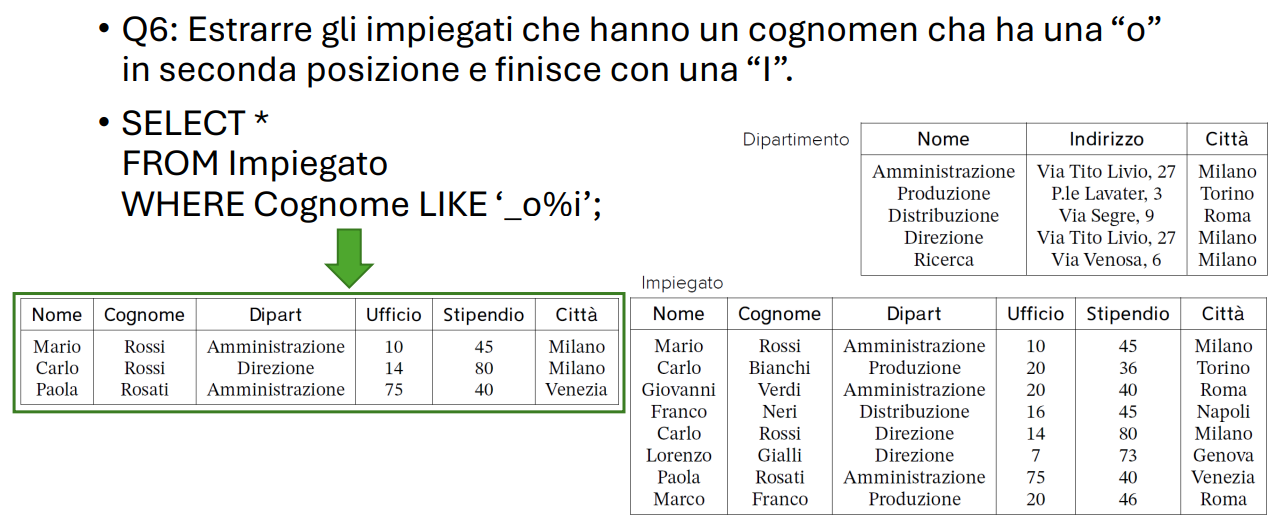
\includegraphics[width=1\linewidth]{image129}
	\caption{Estrarre gli impiegati che hanno un cognomen cha ha una “o” in seconda posizione e finisce con una “I”.}
	\label{fig:image129}
\end{figure}
\subsubsection{Operatore SIMILAR TO}
L'operatore \textbf{SIMILAR TO} è una versione più espressiva dell'operatore \textbf{LIKE}.  
Permette di confrontare stringhe utilizzando un \textbf{pattern} basato su un sottoinsieme delle 
\textbf{espressioni regolari POSIX} nella versione prevista dallo standard SQL.

Questo operatore consente quindi di effettuare confronti più avanzati rispetto a \texttt{LIKE}, 
utilizzando operatori tipici delle espressioni regolari.

\begin{itemize}
	
	\item \texttt{\_} : rappresenta \textbf{un singolo carattere qualsiasi}.
	
	\item \texttt{\%} : rappresenta \textbf{una sequenza di zero o più caratteri qualsiasi}.
	
	\item \texttt{*} : indica la \textbf{ripetizione del match precedente zero o più volte}.
	
	\item \texttt{+} : indica la \textbf{ripetizione del match precedente una o più volte}.
	
	\item \texttt{\{n,m\}} : indica la \textbf{ripetizione del match precedente almeno $n$ volte e al massimo $m$ volte}.
	
	\item \texttt{[...]} : rappresenta un \textbf{insieme di caratteri ammessi}; il match è valido se il carattere appartiene all'insieme specificato.
	
\end{itemize}
\begin{figure}[H]
	\centering
	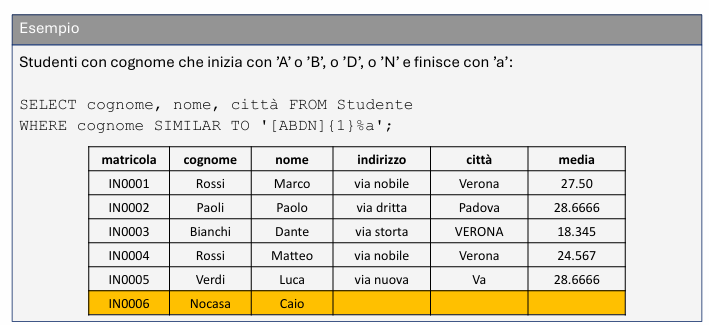
\includegraphics[width=1\linewidth]{image130}
	\caption{Esempio SIMILAR TO}
	\label{fig:image130}
\end{figure}
\subsubsection{Operatore BETWEEN}
L'operatore \textbf{BETWEEN} permette di verificare se il valore di un attributo  è compreso tra due valori estremi.
\begin{figure}[H]
	\centering
	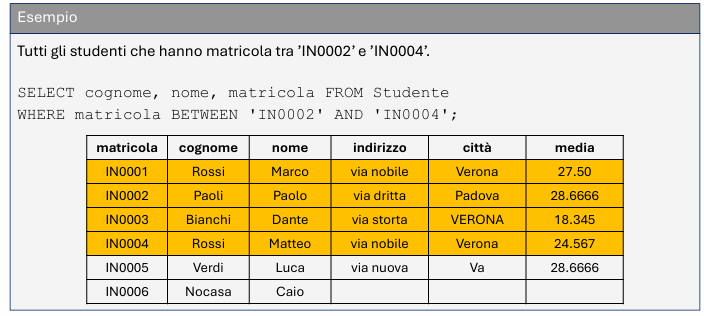
\includegraphics[width=1\linewidth]{image131}
	\caption{Esempio Between}
	\label{fig:image131}
\end{figure}
\begin{figure}[H]
	\centering
	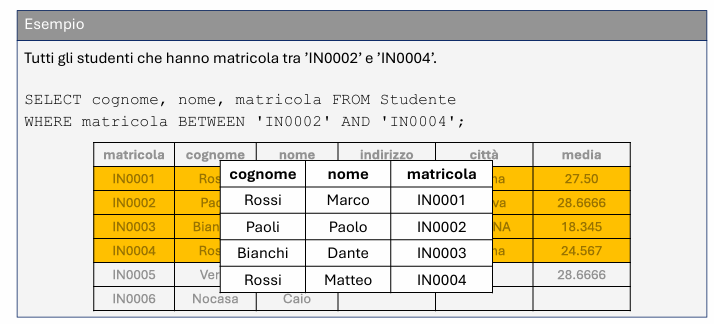
\includegraphics[width=1\linewidth]{image132}
	\caption{Esempio 2 di Between}
	\label{fig:image132}
\end{figure}
\subsubsection{Operatore IN}
Nella clausola \textbf{WHERE} può essere utilizzato l'operatore \textbf{[NOT] IN} 
per verificare se il valore di un attributo appartiene ad un insieme di valori.
\begin{figure}[H]
	\centering
	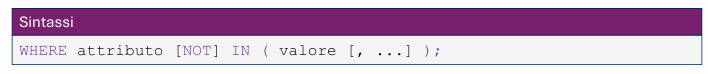
\includegraphics[width=1\linewidth]{image133}
	\caption{Sintassi IN}
	\label{fig:image133}
\end{figure}
\begin{figure}[H]
	\centering
	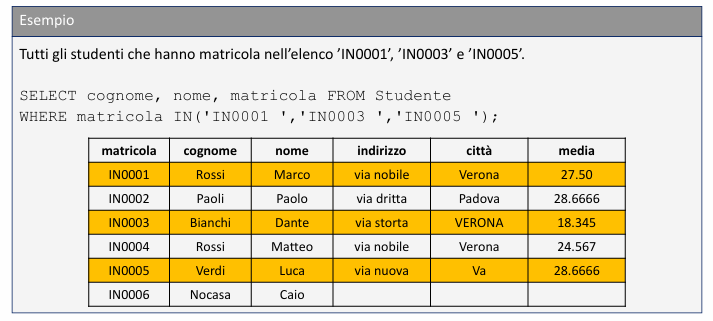
\includegraphics[width=1\linewidth]{image134}
	\caption{Esempio Operatore IN}
	\label{fig:image134}
\end{figure}
\subsubsection{Operatore IS NULL}
Per verificare se un attributo ha un valore nullo oppure no si utilizza il predicato 
\textbf{IS NULL}.

\begin{itemize}
	
	\item \texttt{attributo IS NULL}: restituisce \textbf{true} se l'attributo ha valore nullo.
	
	\item \texttt{attributo IS NOT NULL}: è la negazione del predicato precedente e restituisce 
	\textbf{true} se l'attributo ha un valore diverso da \texttt{NULL}.
	
\end{itemize}
\begin{figure}[H]
	\centering
	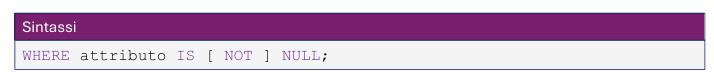
\includegraphics[width=1\linewidth]{image135}
	\caption{Sintassi IS NULL}
	\label{fig:image135}
\end{figure}
\begin{figure}[H]
	\centering
	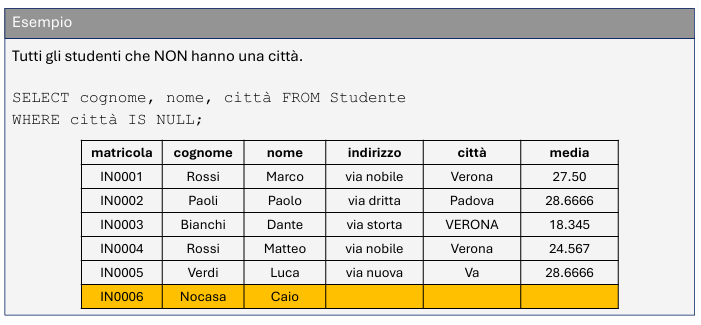
\includegraphics[width=1\linewidth]{image136}
	\caption{Esempio IS NULL}
	\label{fig:image136}
\end{figure}
\subsection{SQL e Algebra Relazionale}
Vediamo ora alcuni esempi di interrogazioni in \textbf{SQL} e analizziamo 
la loro corrispondenza con le equivalenti interrogazioni procedurali 
espresse tramite l'\textbf{algebra relazionale}.

L'obiettivo è comprendere come le interrogazioni dichiarative scritte in SQL 
possano essere interpretate come una sequenza di operazioni dell'algebra 
relazionale, che descrivono in modo procedurale i passi necessari per 
ottenere il risultato desiderato.
\begin{figure}[H]
	\centering
	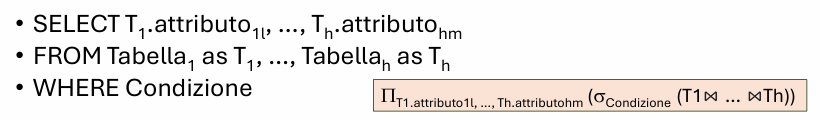
\includegraphics[width=1\linewidth]{image137}
	\caption{Sintassi algebra relazione e sql}
	\label{fig:image137}
\end{figure}
Nel caso di condizioni più complesse, la formula di conversione tra una
interrogazione \textbf{SQL} e la corrispondente espressione in
\textbf{algebra relazionale} non è sempre direttamente rappresentabile.

Una condizione fondamentale per poter effettuare questa conversione è
che l'interrogazione SQL utilizzi solo operatori che esistono anche
nell'algebra relazionale.

Se l'interrogazione SQL utilizza operatori non presenti nell'algebra
relazionale (ad esempio \textbf{operatori aggregati} come
\texttt{COUNT}, \texttt{SUM}, \texttt{AVG}, ecc.), la conversione
diretta non è possibile.
\begin{figure}[H]
	\centering
	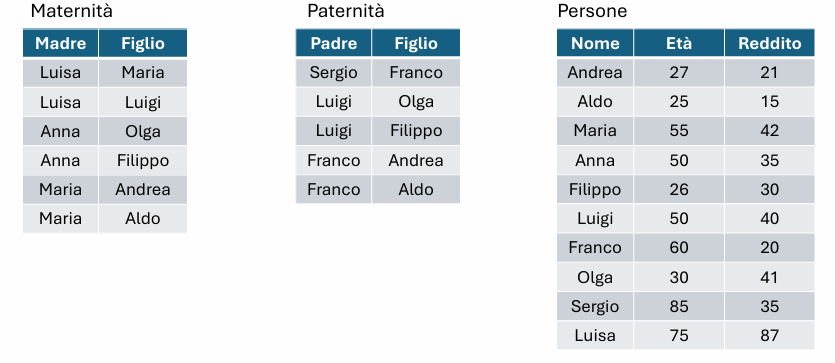
\includegraphics[width=1\linewidth]{image138}
	\caption{Tabella usata per gli esempi}
	\label{fig:image138}
\end{figure}
\subsection{SELECT}
\begin{figure}[H]
	\centering
	
\includegraphics[width=1\linewidth]{image139}
	\caption{}
	\label{fig:image139}
\end{figure}
\subsubsection{SELECT : alias di tabella o di attributo}
\begin{figure}[H]
	\centering
	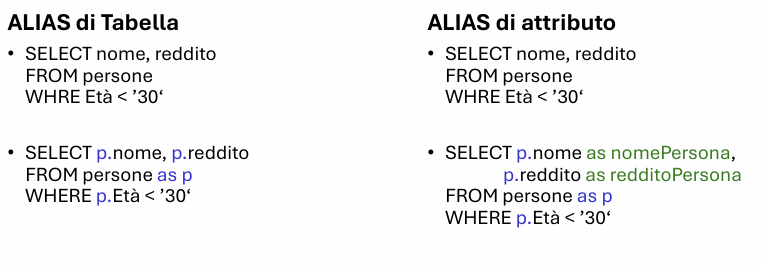
\includegraphics[width=1\linewidth]{image140}
	\caption{SELECT : alias di tabella o di attributo}
	\label{fig:image140}
\end{figure}
\subsubsection{SELECT: senza proiezione}
\begin{figure}[H]
	\centering
	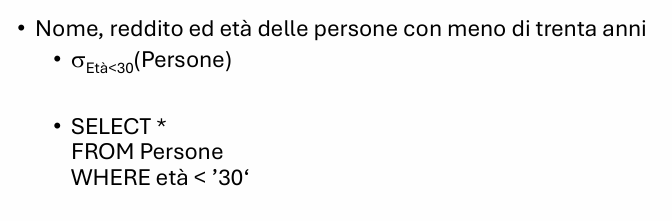
\includegraphics[width=1\linewidth]{image141}
	\caption{SELECT senza proiezione}
	\label{fig:image141}
\end{figure}
\subsubsection{Proiezione:gestione dei duplicati in SQL}

Una differenza significativa tra \textbf{SQL} e l'\textbf{algebra relazionale}
riguarda la gestione dei duplicati.

Nell'algebra relazionale i risultati delle operazioni sono considerati
\textbf{insiemi} e quindi non possono contenere duplicati.
In SQL, invece, i risultati sono trattati come \textbf{multinsiemi}
(\textit{bag}), per cui le righe duplicate possono essere presenti.

L'eliminazione delle righe duplicate è un'operazione computazionalmente
costosa; per questo motivo, \textbf{SQL mantiene i duplicati per default}.

Il costrutto \texttt{DISTINCT}, utilizzato dopo la parola chiave
\texttt{SELECT}, permette di eliminare le righe duplicate dal risultato.

Il costrutto \texttt{ALL} permette invece di mantenere esplicitamente
i duplicati, anche se questa è già la scelta predefinita del linguaggio SQL.
\begin{figure}[H]
	\centering
	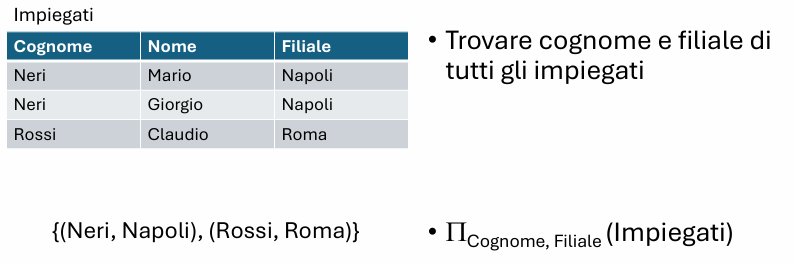
\includegraphics[width=1\linewidth]{image142}
	\caption{Proiezione: gestione dei duplicati in SQL}
	\label{fig:image142}
\end{figure}
\begin{figure}[H]
	\centering
	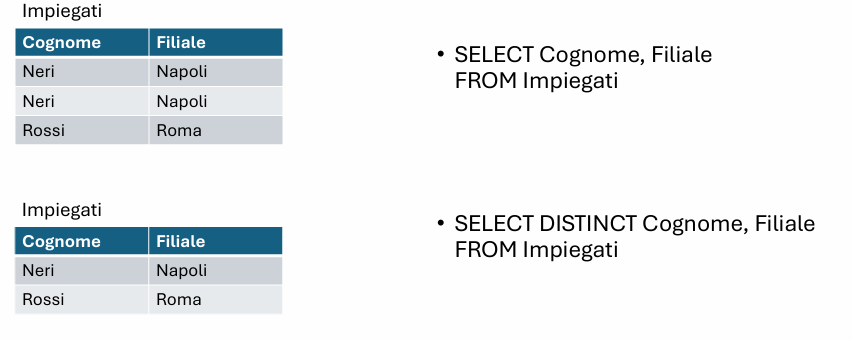
\includegraphics[width=1\linewidth]{image143}
	\caption{}
	\label{fig:image143}
\end{figure}
\begin{figure}[H]
	\centering
	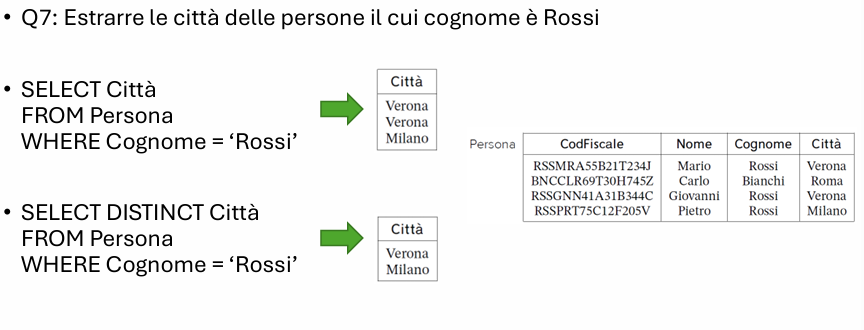
\includegraphics[width=1\linewidth]{image144}
	\caption{Esempio : gestione dei duplicati in SQL}
	\label{fig:image144}
\end{figure}
\subsubsection{SELECT: Selezione,Proiezione,Join}
L'istruzione \textbf{SELECT} permette di esprimere diverse operazioni
dell'\textbf{algebra relazionale}, a seconda della struttura
dell'interrogazione.

\begin{itemize}
	
	\item Con \textbf{una sola relazione} nella clausola \texttt{FROM} è possibile
	realizzare:
	\begin{itemize}
		\item \textbf{selezioni} ($\sigma$)
		\item \textbf{proiezioni} ($\pi$)
		\item \textbf{ridenominazioni} ($\rho$), utilizzando il costrutto \texttt{AS}
	\end{itemize}
	
	\item Con \textbf{più relazioni} nella clausola \texttt{FROM} si possono
	realizzare:
	\begin{itemize}
		\item \textbf{join} ($\bowtie$)
		\item \textbf{prodotti cartesiani}
	\end{itemize}
	
\end{itemize}

Le principali corrispondenze tra le clausole SQL e le operazioni
dell'algebra relazionale sono:

\begin{itemize}
	
	\item \texttt{SELECT} $\rightarrow$ $\pi$ \textbf{Proiezione} + $\rho$ \textbf{Ridenominazione}
	
	\item \texttt{FROM} $\rightarrow$ $\bowtie$ \textbf{Join} (prodotto cartesiano)
	
	\item \texttt{WHERE} $\rightarrow$ $\sigma$ \textbf{Selezione} + $\bowtie$ \textbf{Join} (condizione)
	
\end{itemize}
\subsection{Interrogazioni con JOIN}
In \textbf{SQL} il \textbf{join} può essere definito in due modi diversi.

\begin{itemize}
	
	\item Il primo metodo non richiede l'uso di una nuova sintassi: il legame tra
	le tabelle coinvolte viene specificato nella clausola \texttt{WHERE}.
	
	\item Il secondo metodo utilizza invece una sintassi dedicata all'interno
	della clausola \texttt{FROM}. In questo caso il join viene espresso
	esplicitamente tramite gli operatori di join.
	
\end{itemize}

Nel seguito verrà utilizzato il secondo approccio.
La clausola \textbf{FROM} ammette come argomento:

\begin{center}
	\texttt{table\_name [[AS] name] [, ...]}
\end{center}

Se nella clausola \texttt{FROM} sono presenti due o più nomi di tabelle,
viene eseguito il \textbf{prodotto cartesiano} tra tutte le tabelle.
Lo schema del risultato può quindi contenere tutti gli attributi
derivanti dal prodotto cartesiano delle relazioni coinvolte.

Il prodotto cartesiano tra due o più tabelle è chiamato
\textbf{CROSS JOIN}.

A partire dallo standard \textbf{SQL-2}, sono stati introdotti
altri tipi di join (\textit{join\_type}), tra cui:

\begin{itemize}
	\item \textbf{INNER JOIN}
	\item \textbf{LEFT [OUTER] JOIN}
	\item \textbf{RIGHT [OUTER] JOIN}
	\item \textbf{FULL [OUTER] JOIN}
\end{itemize}
\begin{figure}[H]
	\centering
	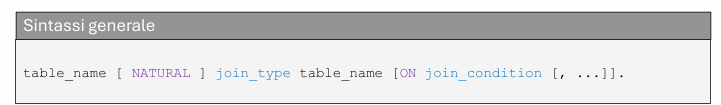
\includegraphics[width=1\linewidth]{image145}
	\caption{Sintassi JOIN}
	\label{fig:image145}
\end{figure}
dove \textit{join\_condition} è un'espressione booleana che seleziona le tuple
del join da aggiungere al risultato.

Le tuple selezionate possono essere successivamente filtrate
mediante la condizione specificata nella clausola \texttt{WHERE}.
\begin{figure}[H]
	\centering
	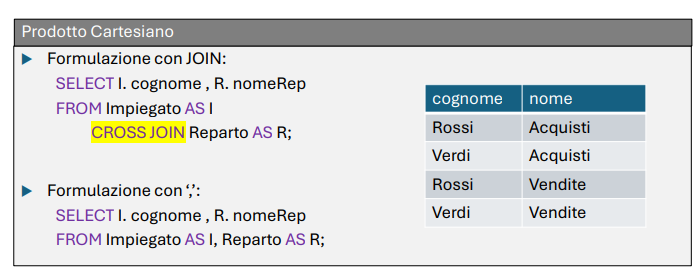
\includegraphics[width=1\linewidth]{image146}
	\caption{Prodotto cartesiano}
	\label{fig:image146}
\end{figure}
\subsubsection{INNER JOIN}
\begin{figure}[H]
	\centering
	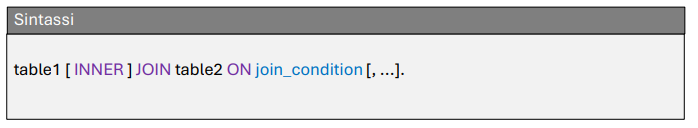
\includegraphics[width=1\linewidth]{image147}
	\caption{Sintassi INNER JOIN}
	\label{fig:image147}
\end{figure}
L'\textbf{INNER JOIN} rappresenta il tradizionale $\theta$-join dell’algebra relazionale.
Combina ciascuna riga $r_1$ della \texttt{table1} con ciascuna riga della \texttt{table2}
che soddisfa la condizione specificata nella clausola \texttt{ON}.
\begin{figure}[H]
	\centering
	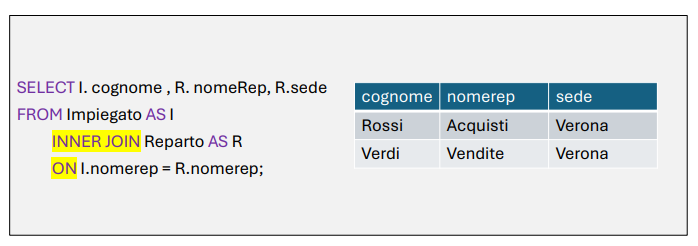
\includegraphics[width=1\linewidth]{image148}
	\caption{Esempio INNER JOIN}
	\label{fig:image148}
\end{figure}
\subsubsection{LEFT OUTER JOIN}
\begin{figure}[H]
	\centering
	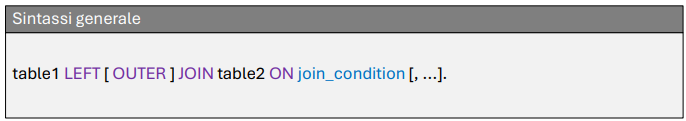
\includegraphics[width=1\linewidth]{image149}
	\caption{Sintassi LEFT OUTER JOIN}
	\label{fig:image149}
\end{figure}
Il \textbf{LEFT OUTER JOIN} esegue prima un \texttt{INNER JOIN}. 
Successivamente, per ogni riga della \texttt{table1} che non trova 
corrispondenza nella \texttt{table2}, viene comunque inserita nel risultato 
una riga contenente i valori della \texttt{table1} e \texttt{NULL} negli 
attributi della \texttt{table2}.
\begin{figure}[H]
	\centering
	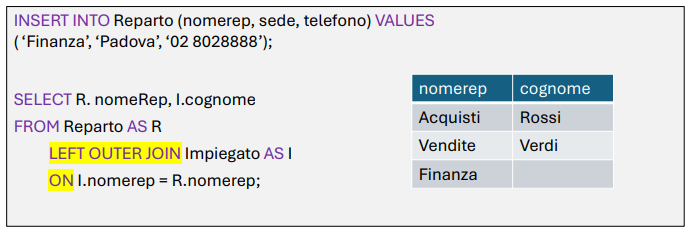
\includegraphics[width=1\linewidth]{image150}
	\caption{Esempio}
	\label{fig:image150}
\end{figure}
\begin{figure}[H]
	\centering
	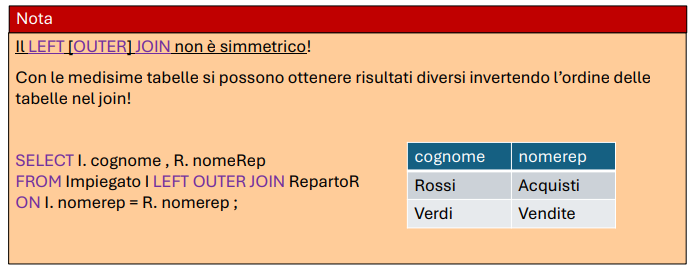
\includegraphics[width=1\linewidth]{image151}
	\caption{Nota}
	\label{fig:image151}
\end{figure}
\subsubsection{RIGHT OUTER JOIN}
\begin{figure}[H]
	\centering
	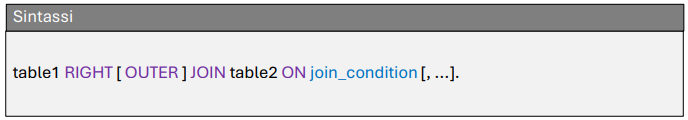
\includegraphics[width=1\linewidth]{image152}
	\caption{Sintassi RIGHT OUTER JOIN}
	\label{fig:image152}
\end{figure}
Il \textbf{RIGHT OUTER JOIN} esegue prima un \texttt{INNER JOIN}. 
Successivamente, per ogni riga della \texttt{table2} che non trova 
corrispondenza nella \texttt{table1}, viene comunque inserita nel risultato 
una riga contenente i valori della \texttt{table2} e \texttt{NULL} negli 
attributi della \texttt{table1}.
\begin{figure}[H]
	\centering
	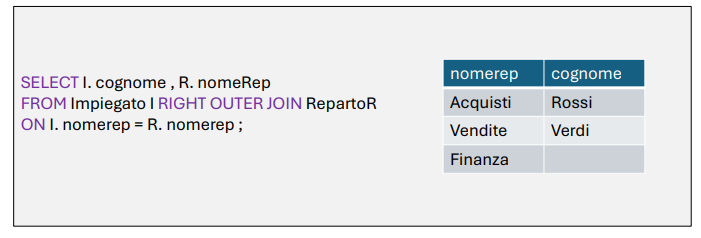
\includegraphics[width=1\linewidth]{image153}
	\caption{Esempio RIGHT OUTER JOIN}
	\label{fig:image153}
\end{figure}
\subsubsection{FULL OUTER JOIN}
\begin{figure}[H]
	\centering
	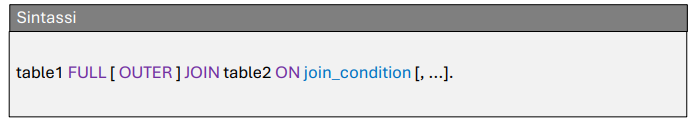
\includegraphics[width=1\linewidth]{image154}
	\caption{FULL OUTER JOIN}
	\label{fig:image154}
\end{figure}
Il \textbf{FULL OUTER JOIN} restituisce tutte le tuple prodotte da un 
\texttt{INNER JOIN}, più le tuple della prima tabella che non trovano 
corrispondenza nella seconda (come nel \texttt{LEFT OUTER JOIN}) e le 
tuple della seconda tabella che non trovano corrispondenza nella prima 
(come nel \texttt{RIGHT OUTER JOIN}). 

Non è equivalente a un \texttt{CROSS JOIN}.
\begin{figure}[H]
	\centering
	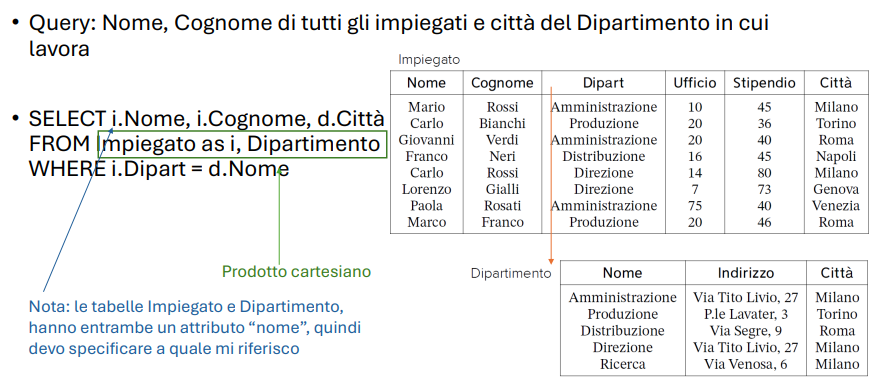
\includegraphics[width=1\linewidth]{image155}
	\caption{Esempio}
	\label{fig:image155}
\end{figure}
Il \textbf{join} può essere specificato direttamente nella clausola
\texttt{FROM}, a livello delle tabelle coinvolte. Nello svolgimento degli
esercizi utilizzeremo questa sintassi dedicata.

\begin{verbatim}
	SELECT ListaAttributi
	FROM Tabella1 JOIN Tabella2 ON (CondizioneDiJoin)
	[WHERE AltraCondizione]
\end{verbatim}

Esempio:

\begin{verbatim}
	SELECT i.Nome, d.Città
	FROM Impiegato AS i JOIN Dipartimento AS d
	ON (i.Dipart = d.Nome)
\end{verbatim}
\textbf{Q8:} Selezionare i padri di persone che guadagnano più di 20.

\medskip

\textbf{Algebra relazionale}

\[
\pi_{Padre} \big( \text{Paternità} \ \bowtie_{Figlio = Nome} \ (\sigma_{Reddito > 20}(\text{Persone})) \big)
\]

\medskip

\textbf{SQL}

\begin{verbatim}
	SELECT DISTINCT Padre
	FROM Persone
	JOIN Paternità ON (Figlio = Nome)
	WHERE Reddito > 20;
\end{verbatim}
\subsection{Uso di variabili (alias)}

SQL permette di associare un \textbf{nome alternativo} (alias) alle tabelle
che compaiono nella clausola \texttt{FROM}.

\begin{itemize}
	\item Il nome alternativo viene utilizzato per fare riferimento alla
	tabella nel contesto dell'interrogazione.
	
	\item L'alias viene definito nella clausola \texttt{FROM} tramite la
	parola chiave \texttt{AS} (opzionale).
\end{itemize}

\textbf{Motivi per usare gli alias:}

\begin{itemize}
	\item Fare riferimento alla tabella in modo più compatto.
	\item Accedere più volte alla stessa tabella all'interno della stessa
	interrogazione (self join).
\end{itemize}
\begin{figure}[H]
	\centering
	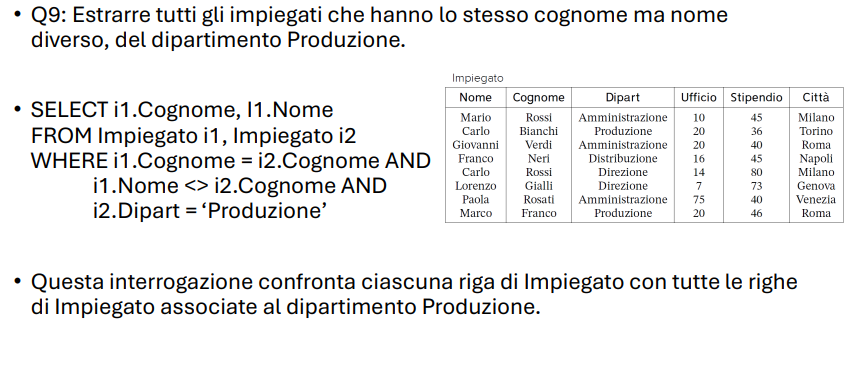
\includegraphics[width=1\linewidth]{image156}
	\caption{Esempio Uso di variabili (alias)}
	\label{fig:image156}
\end{figure}
\begin{itemize}
	\item Si può immaginare che, al momento della definizione degli alias,
	vengano create due copie della tabella \texttt{Impiegato}, ciascuna
	associata a una delle due variabili \texttt{i1} e \texttt{i2}.
	
	\item Le due copie contengono inizialmente tutte le righe della tabella
	\texttt{Impiegato}.
	
	\item Successivamente, sulla copia \texttt{i2} vengono selezionate solo
	le righe relative al dipartimento \texttt{'Produzione'}.
\end{itemize}
\subsection{Ordinamento del risultato}
Come abbiamo visto, una relazione è un insieme di tuple \textbf{non ordinato}.
Nella pratica, però, spesso è necessario visualizzare le righe secondo
un determinato ordine.

SQL permette di specificare un ordinamento (ascendente o discendente)
delle righe dell'output tramite la clausola \texttt{ORDER BY}, che viene
posta alla fine dell'interrogazione.
\begin{figure}[H]
	\centering
	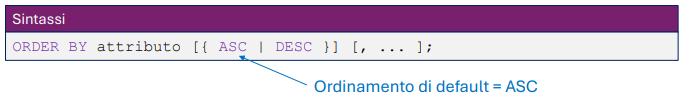
\includegraphics[width=1\linewidth]{image157}
	\caption{Sintassi Ordinamento del risultato}
	\label{fig:image157}
\end{figure}
Se nella clausola \texttt{ORDER BY} sono presenti più attributi, le righe
vengono ordinate rispetto al primo attributo dell'elenco; a parità di valore
del primo attributo si utilizza il secondo, e così via in sequenza.
\begin{figure}[H]
	\centering
	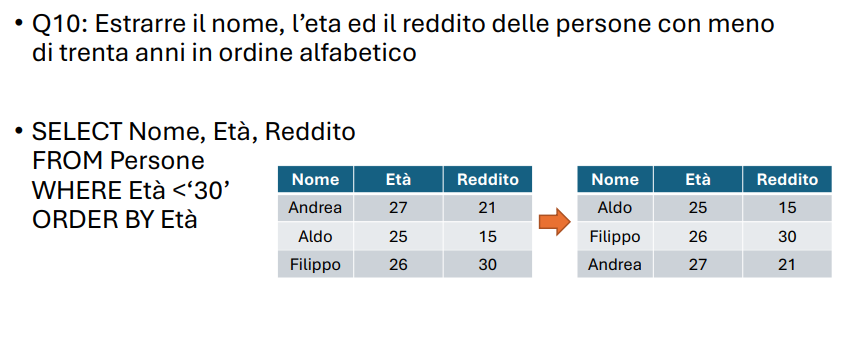
\includegraphics[width=1\linewidth]{image158}
	\caption{Esempio: Ordinamento del risultato}
	\label{fig:image158}
\end{figure}
\begin{figure}[H]
	\centering
	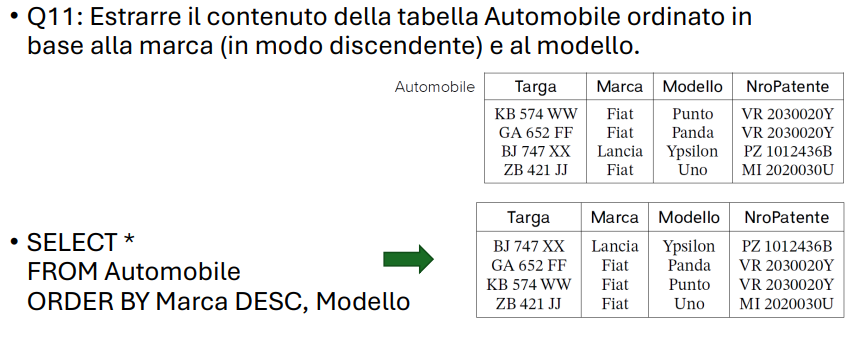
\includegraphics[width=1\linewidth]{image159}
	\caption{Esempio Ordinamento del risultato}
	\label{fig:image159}
\end{figure}
\subsubsection{Operazioni Insiemistiche}
SQL mette a disposizione alcuni \textbf{operatori insiemistici} che permettono
di combinare i risultati di più interrogazioni.

\begin{verbatim}
	SELECT ...
	{ UNION | INTERSECT | EXCEPT [ALL] }
	SELECT ...
\end{verbatim}

\begin{itemize}
	\item Gli operatori insiemistici, a differenza del resto del linguaggio SQL,
	\textbf{eliminano i duplicati per default}. 
	
	\item Se si vogliono mantenere i duplicati è necessario utilizzare la
	parola chiave \texttt{ALL}.
	
	\item Le interrogazioni combinate devono restituire lo stesso
	\textbf{numero di attributi} e avere \textbf{domini compatibili}.
	
	\item La corrispondenza tra gli attributi avviene per \textbf{posizione}
	(ordine posizionale), non per nome.
	
	\item Se i nomi degli attributi sono diversi, di solito il sistema utilizza
	il nome degli attributi del \textbf{primo operando}.
\end{itemize}
\subsubsection{Unione}
\begin{figure}[H]
	\centering
	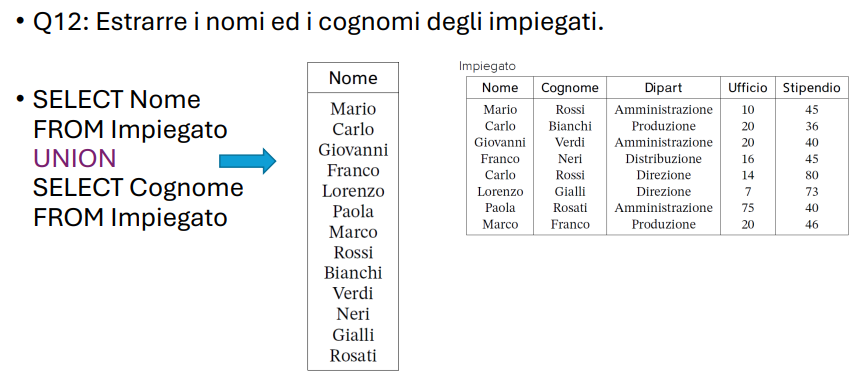
\includegraphics[width=1\linewidth]{image160}
	\caption{Esempio Unione}
	\label{fig:image160}
\end{figure}
\begin{figure}[H]
	\centering
	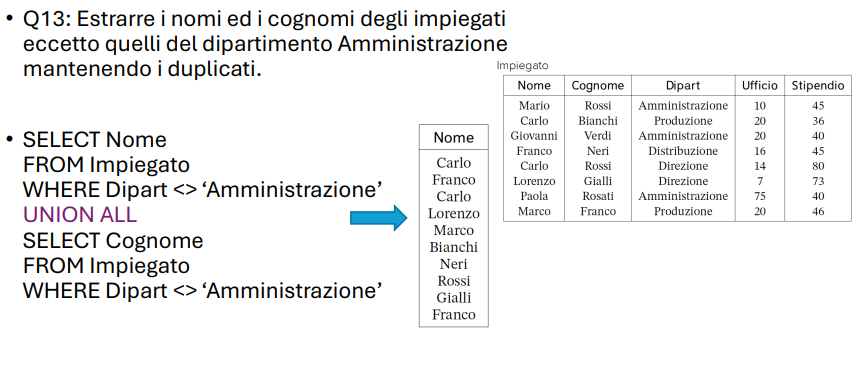
\includegraphics[width=1\linewidth]{image161}
	\caption{Esempio Unione}
	\label{fig:image161}
\end{figure}
\subsubsection{Intersezione}
\begin{figure}[H]
	\centering
	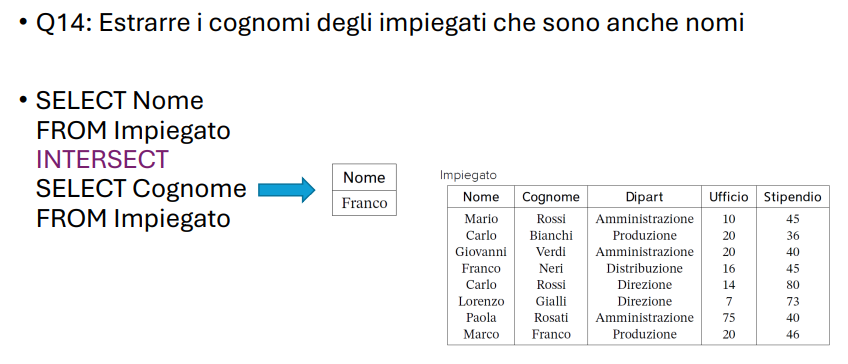
\includegraphics[width=1\linewidth]{image162}
	\caption{Intersezione}
	\label{fig:image162}
\end{figure}
\subsubsection{Differenza}
\begin{figure}[H]
	\centering
	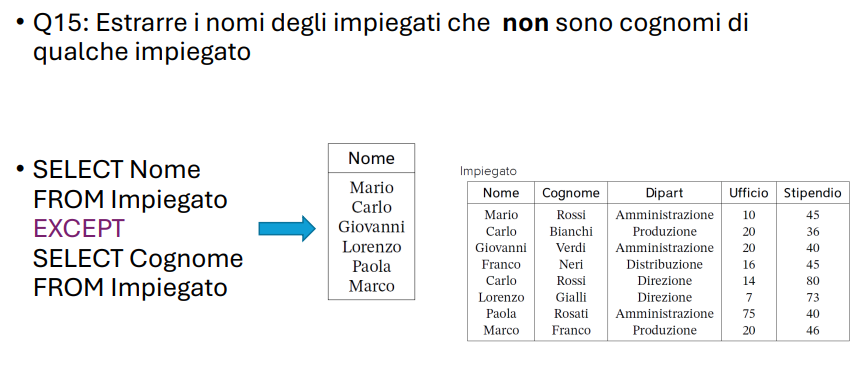
\includegraphics[width=1\linewidth]{image163}
	\caption{Differenza}
	\label{fig:image163}
\end{figure}
\subsection{Operatori aggregati}

Gli operatori di aggregazione rappresentano una delle più importanti
estensioni di SQL rispetto all'algebra relazionale.

\begin{itemize}
	\item I principali operatori di aggregazione sono:
	\texttt{COUNT}, \texttt{SUM}, \texttt{MAX}, \texttt{MIN} e \texttt{AVG}.
	
	\item Nell'algebra relazionale tutte le condizioni specificate vengono
	valutate su \textbf{una tupla alla volta}.
	
	\item Gli operatori di aggregazione, invece, permettono di valutare
	proprietà che dipendono da \textbf{insiemi di tuple}.
	
	\item Prima viene eseguita l'interrogazione considerando solo le
	clausole \texttt{FROM} e \texttt{WHERE}.
	
	\item Successivamente l'operatore di aggregazione viene applicato
	alla tabella contenente il risultato dell'interrogazione.
\end{itemize}
\subsubsection{COUNT}
L'operatore \texttt{COUNT} conta il numero di righe di una tabella oppure
il numero di valori di uno o più attributi.

\begin{verbatim}
	COUNT ( <* | [DISTINCT | ALL] ListaAttributi> )
\end{verbatim}

\begin{itemize}
	\item \texttt{*}: conta il numero totale di righe della tabella.
	
	\item \texttt{DISTINCT ListaAttributi}: conta il numero di valori
	\textbf{distinti} degli attributi specificati.
	
	\item \texttt{ALL ListaAttributi}: conta il numero di righe che hanno
	valori \textbf{diversi da NULL} negli attributi indicati.
	
	\item \texttt{ALL} rappresenta il \textbf{comportamento di default}.
\end{itemize}
\begin{figure}[H]
	\centering
	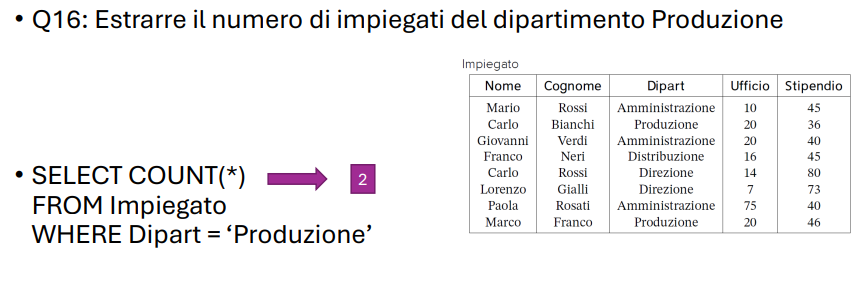
\includegraphics[width=1\linewidth]{image164}
	\caption{Esempio COUNT}
	\label{fig:image164}
\end{figure}
\begin{figure}[H]
	\centering
	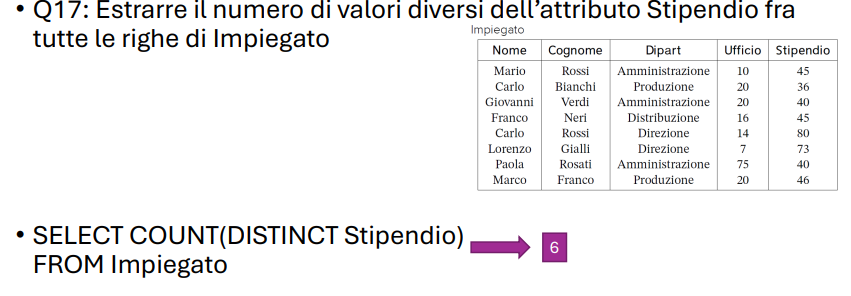
\includegraphics[width=1\linewidth]{image165}
	\caption{Esempio Count}
	\label{fig:image165}
\end{figure}
\begin{figure}[H]
	\centering
	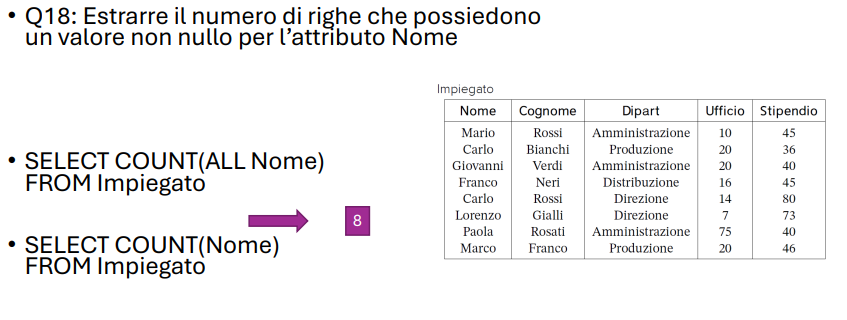
\includegraphics[width=1\linewidth]{image166}
	\caption{Esempio Count}
	\label{fig:image166}
\end{figure}
\subsubsection{Operatori aggregati: SUM.MAX,MIN,AVG}
\begin{verbatim}
	<SUM | MAX | MIN | AVG> ( [DISTINCT | ALL] AttrExpr )
\end{verbatim}

\begin{itemize}
	\item \texttt{SUM}: restituisce la somma dei valori posseduti
	dall'espressione.
	
	\item \texttt{MAX} / \texttt{MIN}: restituiscono rispettivamente il
	valore massimo o minimo tra quelli posseduti dall'espressione.
	
	\item \texttt{AVG}: restituisce la media dei valori.
	
	\item \texttt{SUM} e \texttt{AVG} ammettono come argomento solo
	espressioni che rappresentano valori \textbf{numerici} o
	\textbf{intervalli di tempo}.
	
	\item \texttt{MAX} e \texttt{MIN} ammettono come argomento
	espressioni su cui è definito un \textbf{ordinamento}
	(ad esempio anche stringhe).
	
	\item \texttt{DISTINCT} elimina i valori duplicati prima
	dell'applicazione dell'operatore.
	
	\item \texttt{ALL} considera tutti i valori, \textbf{trascurando solo
		i valori NULL}. Questo è il comportamento di default.
	
	\item \texttt{DISTINCT} e \texttt{ALL} non hanno effetto sugli
	operatori \texttt{MIN} e \texttt{MAX}.
\end{itemize}
\begin{figure}[H]
	\centering
	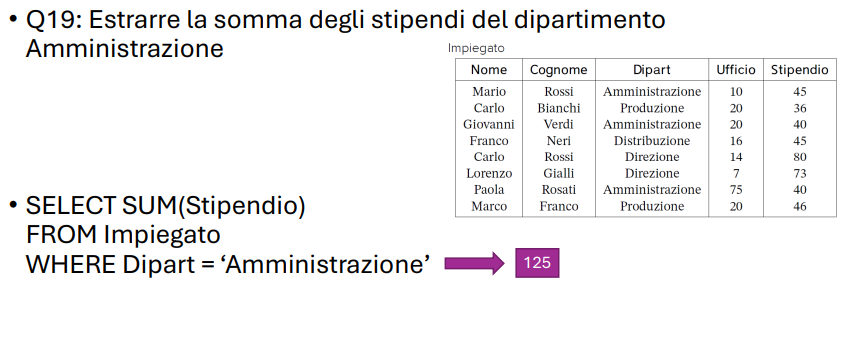
\includegraphics[width=1\linewidth]{image167}
	\caption{Esempio SUM}
	\label{fig:image167}
\end{figure}
\begin{figure}[H]
	\centering
	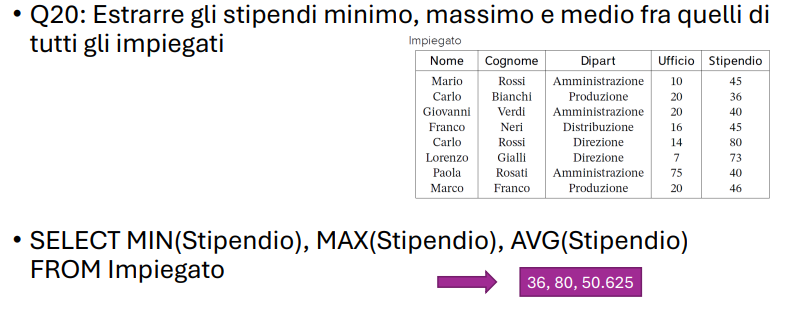
\includegraphics[width=1\linewidth]{image168}
	\caption{Esempio MAX,MIN,AVG}
	\label{fig:image168}
\end{figure}
\begin{figure}[H]
	\centering
	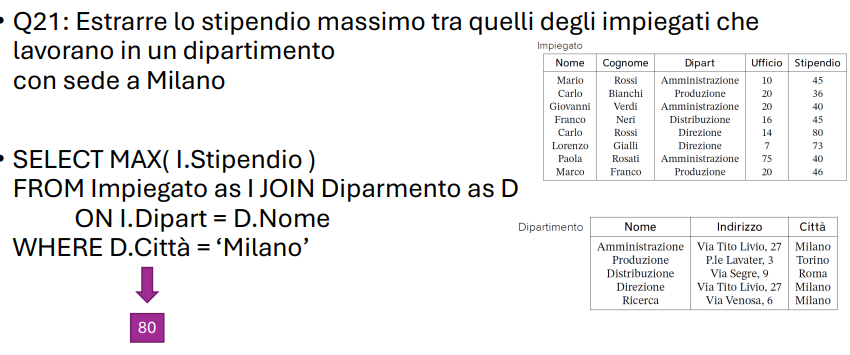
\includegraphics[width=1\linewidth]{image169}
	\caption{Esempio MAX}
	\label{fig:image169}
\end{figure}
\begin{verbatim}
	SELECT Cognome, Nome, MAX(I.Stipendio)
	FROM Impiegato AS I JOIN Dipartimento AS D
	ON I.Dipart = D.Nome
	WHERE D.Città = 'Milano'
\end{verbatim}

\begin{itemize}
	\item La seguente interrogazione non è corretta.
	
	\item Gli operatori di aggregazione non sono un meccanismo di selezione,
	ma funzioni che restituiscono un valore quando vengono applicate
	a un insieme di tuple.
	
	\item Gli attributi \texttt{Cognome} e \texttt{Nome} restituiscono
	un valore per \textbf{ogni tupla selezionata}, mentre
	\texttt{MAX()} restituisce un \textbf{unico valore} per
	l'intero insieme.
	
	\item Si crea quindi un'incoerenza tra attributi normali
	e funzione di aggregazione.
	
	\item Per risolvere questa situazione è necessario utilizzare
	il meccanismo di \textbf{raggruppamento} tramite la clausola
	\texttt{GROUP BY}.
\end{itemize}
\subsection{Interrogazioni con raggruppamento}
Gli operatori di aggregazione possono essere applicati separatamente
a \textbf{sottoinsiemi di righe}.

\begin{itemize}
	\item La clausola \texttt{GROUP BY} permette di specificare come
	dividere le righe della tabella in sottoinsiemi.
	
	\item La clausola consente di indicare un insieme di attributi
	rispetto ai quali effettuare il raggruppamento.
	
	\item L'interrogazione raggruppa quindi tutte le righe che
	possiedono gli \textbf{stessi valori} per tali attributi.
\end{itemize}
\begin{figure}[H]
	\centering
	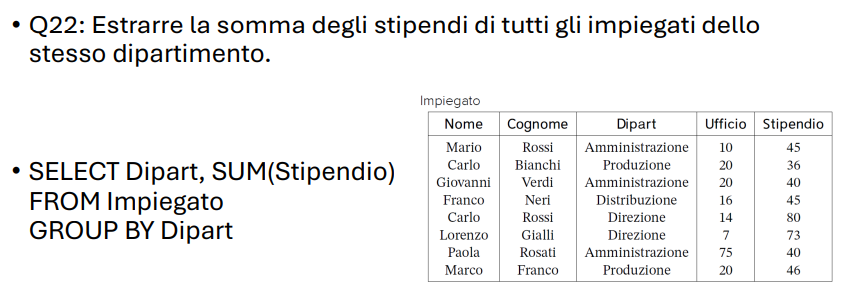
\includegraphics[width=1\linewidth]{image170}
	\caption{Esempio GROUP BY}
	\label{fig:image170}
\end{figure}
\begin{figure}[H]
	\centering
	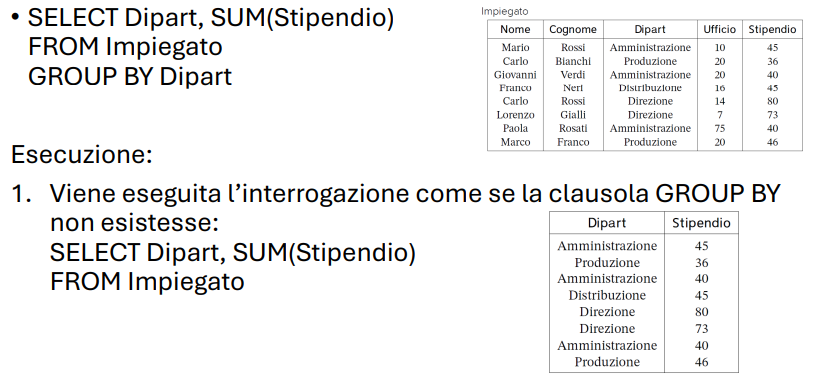
\includegraphics[width=1\linewidth]{image171}
	\caption{Esempio GROUP BY}
	\label{fig:image171}
\end{figure}
\begin{figure}[H]
	\centering
	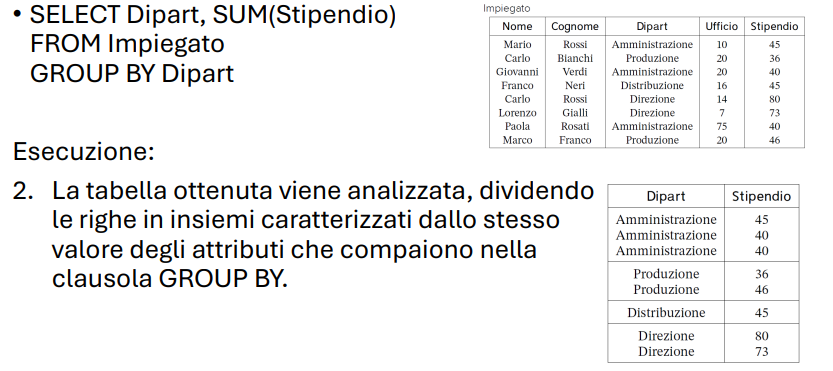
\includegraphics[width=1\linewidth]{image172}
	\caption{Esempio GROUP BY}
	\label{fig:image172}
\end{figure}
\begin{figure}[H]
	\centering
	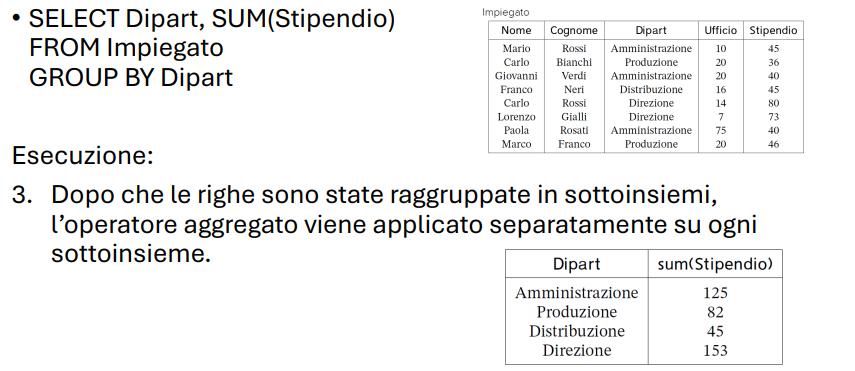
\includegraphics[width=1\linewidth]{image173}
	\caption{Esempio GROUP BY}
	\label{fig:image173}
\end{figure}
In una interrogazione che utilizza la clausola \texttt{GROUP BY}, nella
clausola \texttt{SELECT} possono comparire solo:

\begin{itemize}
	\item attributi che appartengono all'insieme specificato nella
	clausola \texttt{GROUP BY};
	\item oppure operatori di aggregazione.
\end{itemize}

\textbf{Esempio di interrogazione non corretta}

\begin{verbatim}
	SELECT Ufficio
	FROM Impiegato
	GROUP BY Dipart
\end{verbatim}

\textbf{Errore:}

\begin{itemize}
	\item Ad ogni valore dell'attributo \texttt{Dipart} possono
	corrispondere diversi valori dell'attributo \texttt{Ufficio}.
	
	\item Ogni sottoinsieme di righe generato dal \texttt{GROUP BY}
	deve corrispondere ad \textbf{una sola riga} nella tabella
	risultato.
\end{itemize}
\subsubsection{HAVING}
È possibile applicare delle \textbf{selezioni ai gruppi} generati tramite
la clausola \texttt{GROUP BY}.

\begin{itemize}
	\item La clausola \texttt{HAVING} permette di specificare condizioni
	che devono essere soddisfatte dai \textbf{gruppi di tuple} generati
	dopo l'esecuzione del raggruppamento tramite \texttt{GROUP BY}.
	
	\item A differenza della clausola \texttt{WHERE}, che filtra le
	\textbf{singole tuple} prima del raggruppamento, la clausola
	\texttt{HAVING} filtra i \textbf{gruppi} dopo il raggruppamento.
\end{itemize}

\textbf{Esempio}

\begin{verbatim}
	SELECT Dipart, SUM(Stipendio) AS SommaStipendi
	FROM Impiegato
	GROUP BY Dipart
	HAVING SUM(Stipendio) > 100;
\end{verbatim}
\begin{figure}[H]
	\centering
	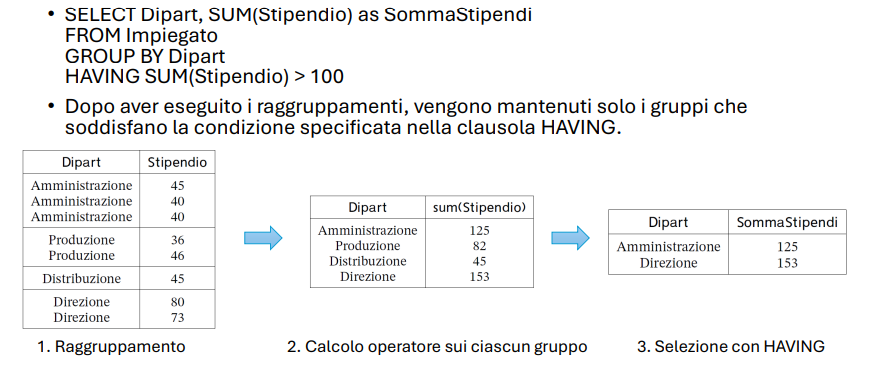
\includegraphics[width=1\linewidth]{image174}
	\caption{HAVING + GROUP BY}
	\label{fig:image174}
\end{figure}
\begin{itemize}
	\item La clausola \texttt{WHERE} applica delle selezioni su
	\textbf{singole righe}, prima dell'eventuale raggruppamento
	tramite \texttt{GROUP BY}.
	
	\item La clausola \texttt{HAVING} applica delle selezioni su
	\textbf{gruppi di righe}, generati dopo l'esecuzione del
	raggruppamento tramite \texttt{GROUP BY}.
\end{itemize}

\textbf{Esempio}

\begin{verbatim}
	SELECT Dipart
	FROM Impiegato
	WHERE Ufficio = 20
	GROUP BY Dipart
	HAVING AVG(Stipendio) > 25;
\end{verbatim}

\textbf{Ordine logico di esecuzione}

\begin{enumerate}
	\item \texttt{WHERE} → seleziona le righe che verranno raggruppate.
	\item \texttt{GROUP BY} → forma i gruppi con le righe selezionate.
	\item \texttt{HAVING} → seleziona i gruppi che faranno parte del risultato.
\end{enumerate}
\subsection{Interrogazioni nidificate}
Una \textbf{interrogazione nidificata} è una interrogazione SQL che
contiene al suo interno una o più interrogazioni.

\begin{itemize}
	\item La nidificazione può avvenire nella clausola \texttt{SELECT},
	nella clausola \texttt{FROM} oppure nella clausola \texttt{WHERE}.
	
	\item Il caso più comune è la nidificazione nella clausola
	\texttt{WHERE}.
	
	\item In questo caso un predicato contiene un confronto tra
	un valore (un'espressione valutata su una singola riga) e
	il risultato di un'altra interrogazione SQL.
\end{itemize}
Quando in un predicato si confronta un attributo (o un'espressione che
produce un valore singolo) con il risultato di un'interrogazione,
può sorgere un problema di disomogeneità tra i termini del confronto,
poiché la sottointerrogazione può restituire più valori.

\begin{itemize}
	\item I normali operatori di confronto
	(\texttt{=}, \texttt{<>}, \texttt{<}, \texttt{>}, \texttt{<=}, \texttt{>=})
	possono essere estesi con le parole chiave \texttt{ANY} e \texttt{ALL}.
	
	\item \texttt{ANY}: la riga soddisfa la condizione se il confronto
	tra il valore dell'attributo (o dell'espressione) e \textbf{almeno
		uno} dei valori restituiti dalla sottointerrogazione risulta vero.
	
	\item \texttt{ALL}: la riga soddisfa la condizione se il confronto
	tra il valore dell'attributo (o dell'espressione) e \textbf{tutti}
	i valori restituiti dalla sottointerrogazione risulta vero.
\end{itemize}
\begin{figure}[H]
	\centering
	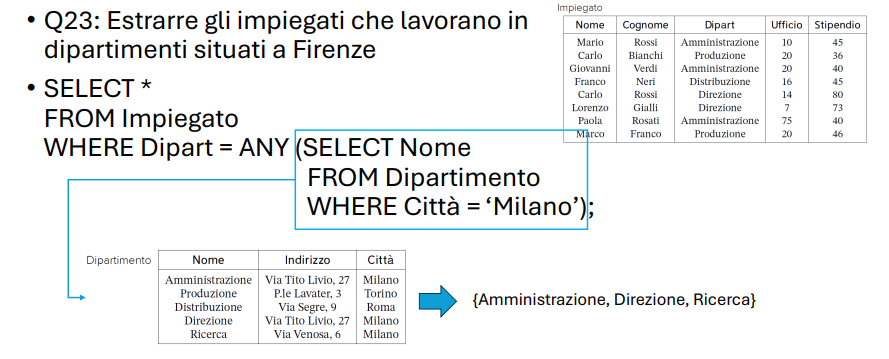
\includegraphics[width=1\linewidth]{image175}
	\caption{WHERE}
	\label{fig:image175}
\end{figure}
\begin{figure}[H]
	\centering
	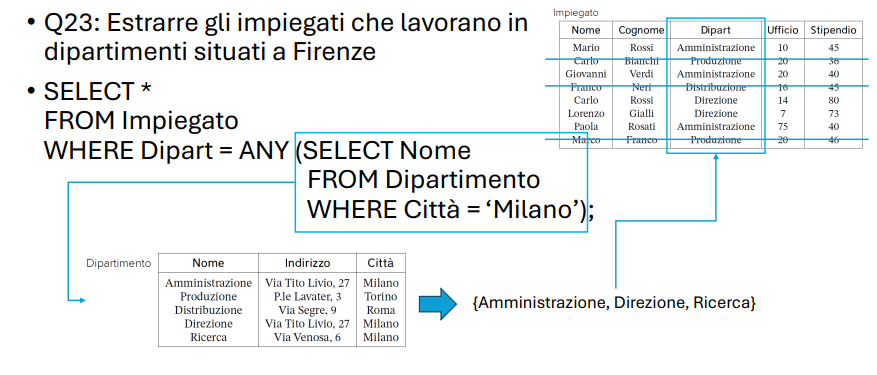
\includegraphics[width=1\linewidth]{image176}
	\caption{}
	\label{fig:image176}
\end{figure}
\begin{figure}[H]
	\centering
	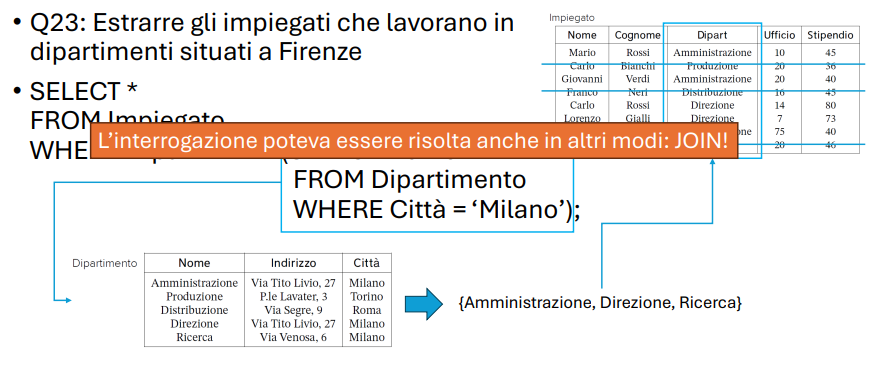
\includegraphics[width=1\linewidth]{image177}
	\caption{}
	\label{fig:image177}
\end{figure}
\begin{figure}[H]
	\centering
	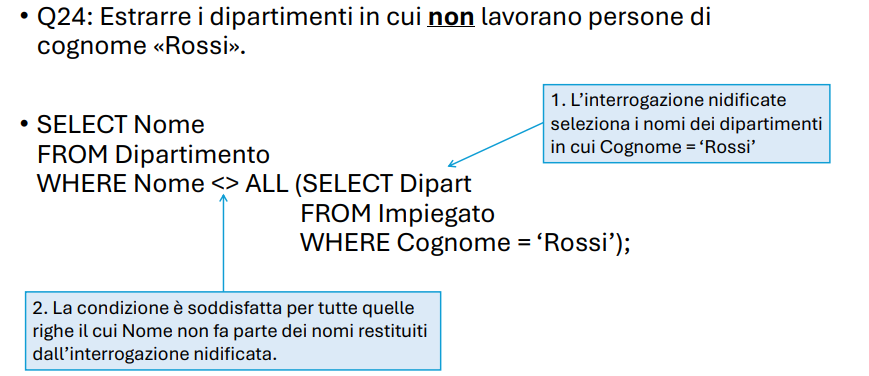
\includegraphics[width=1\linewidth]{image178}
	\caption{}
	\label{fig:image178}
\end{figure}
\textbf{Esempio con ALL}

\begin{verbatim}
	SELECT Nome
	FROM Dipartimento
	WHERE Nome <> ALL
	(SELECT Dipart
	FROM Impiegato
	WHERE Cognome = 'Rossi');
\end{verbatim}

Questa interrogazione seleziona i dipartimenti il cui nome è
\textbf{diverso da tutti} i valori restituiti dalla sottointerrogazione,
cioè i dipartimenti in cui non lavora nessun impiegato con cognome
\texttt{'Rossi'}.

\medskip

\textbf{Interrogazione equivalente}

\begin{verbatim}
	SELECT Nome
	FROM Dipartimento
	EXCEPT
	SELECT Dipart
	FROM Impiegato
	WHERE Cognome = 'Rossi';
\end{verbatim}
Per le interrogazioni nidificate viste fino ad ora, la sottointerrogazione
può essere eseguita \textbf{una sola volta} e il risultato ottenuto può
essere salvato in una \textbf{tabella temporanea}, utilizzata per
eseguire i confronti con le righe della tabella esterna.

\begin{itemize}
	\item In alcuni casi, però, la sottointerrogazione fa riferimento
	al contesto dell'interrogazione esterna tramite l'uso di una
	variabile (passaggio di \textit{binding}).
	
	\item In questo caso si parla di \textbf{interrogazione nidificata
		correlata}.
	
	\item La sottointerrogazione deve essere quindi valutata
	\textbf{separatamente per ogni riga} prodotta
	dall'interrogazione esterna.
\end{itemize}
L'operatore logico \texttt{EXISTS} riceve come parametro
un'interrogazione nidificata e restituisce il valore \textbf{vero}
solo se la sottointerrogazione produce un risultato \textbf{non vuoto}.

\begin{itemize}
	\item Se la sottointerrogazione restituisce almeno una riga,
	la condizione \texttt{EXISTS} risulta vera.
	
	\item Se la sottointerrogazione non restituisce alcuna riga,
	la condizione \texttt{EXISTS} risulta falsa.
	
	\item Questo operatore è particolarmente utile quando esiste
	un \textbf{passaggio di binding} tra la query esterna e la
	sottointerrogazione.
\end{itemize}
\begin{figure}[H]
	\centering
	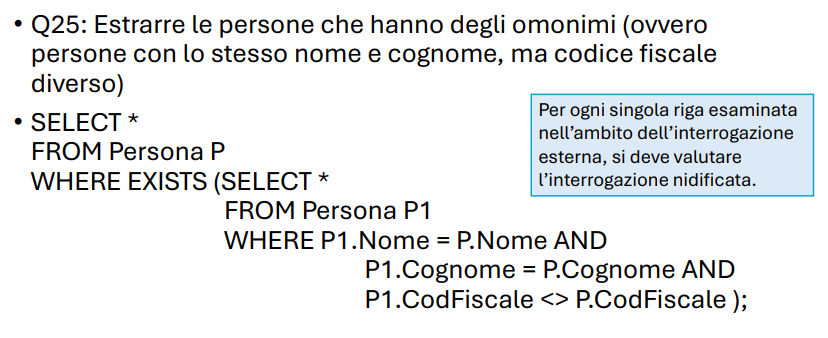
\includegraphics[width=1\linewidth]{image179}
	\caption{}
	\label{fig:image179}
\end{figure}
\begin{figure}[H]
	\centering
	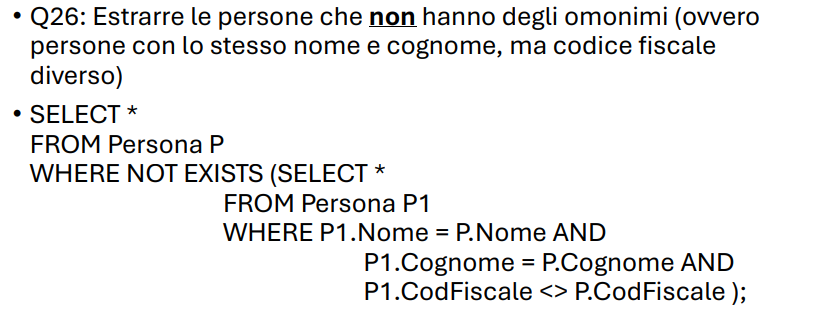
\includegraphics[width=1\linewidth]{image180}
	\caption{}
	\label{fig:image180}
\end{figure}
\begin{figure}[H]
	\centering
	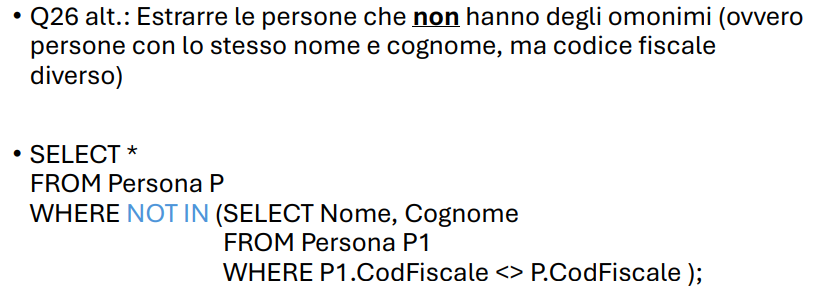
\includegraphics[width=1\linewidth]{image181}
	\caption{}
	\label{fig:image181}
\end{figure}
\begin{figure}[H]
	\centering
	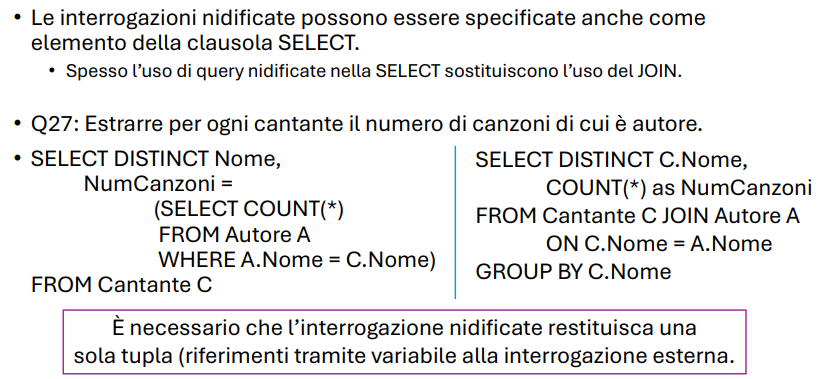
\includegraphics[width=1\linewidth]{image182}
	\caption{}
	\label{fig:image182}
\end{figure}
Le interrogazioni nidificate possono essere utilizzate nella
clausola \texttt{FROM} come sorgenti di dati su cui eseguire
l'interrogazione principale.

\begin{itemize}
	\item È possibile creare una \textbf{catena di interrogazioni},
	in cui ogni interrogazione utilizza il risultato della
	precedente come se fosse una tabella di base.
	
	\item In questo modo il risultato di una sottointerrogazione
	viene trattato come una \textbf{tabella temporanea}.
\end{itemize}

\textbf{Q28:} Estrarre per ogni cantante che è anche autore di canzoni
il numero di canzoni di cui è rispettivamente interprete e autore.

\begin{verbatim}
	SELECT DISTINCT C.Nome, C.NumCantate, A.NumScritte
	FROM
	(SELECT Nome, COUNT(*) AS NumCantate
	FROM Cantante
	GROUP BY Nome) C
	JOIN
	(SELECT Nome, COUNT(*) AS NumScritte
	FROM Autore
	GROUP BY Nome) A
	ON C.Nome = A.Nome;
\end{verbatim}

\begin{itemize}
	\item Prima vengono eseguite le interrogazioni presenti nella
	clausola \texttt{FROM}.
	
	\item I risultati ottenuti vengono poi utilizzati come
	\textbf{normali tabelle} nell'interrogazione esterna.
\end{itemize}